% Created by tikzDevice version 0.12.4 on 2024-12-11 15:47:26
% !TEX encoding = UTF-8 Unicode
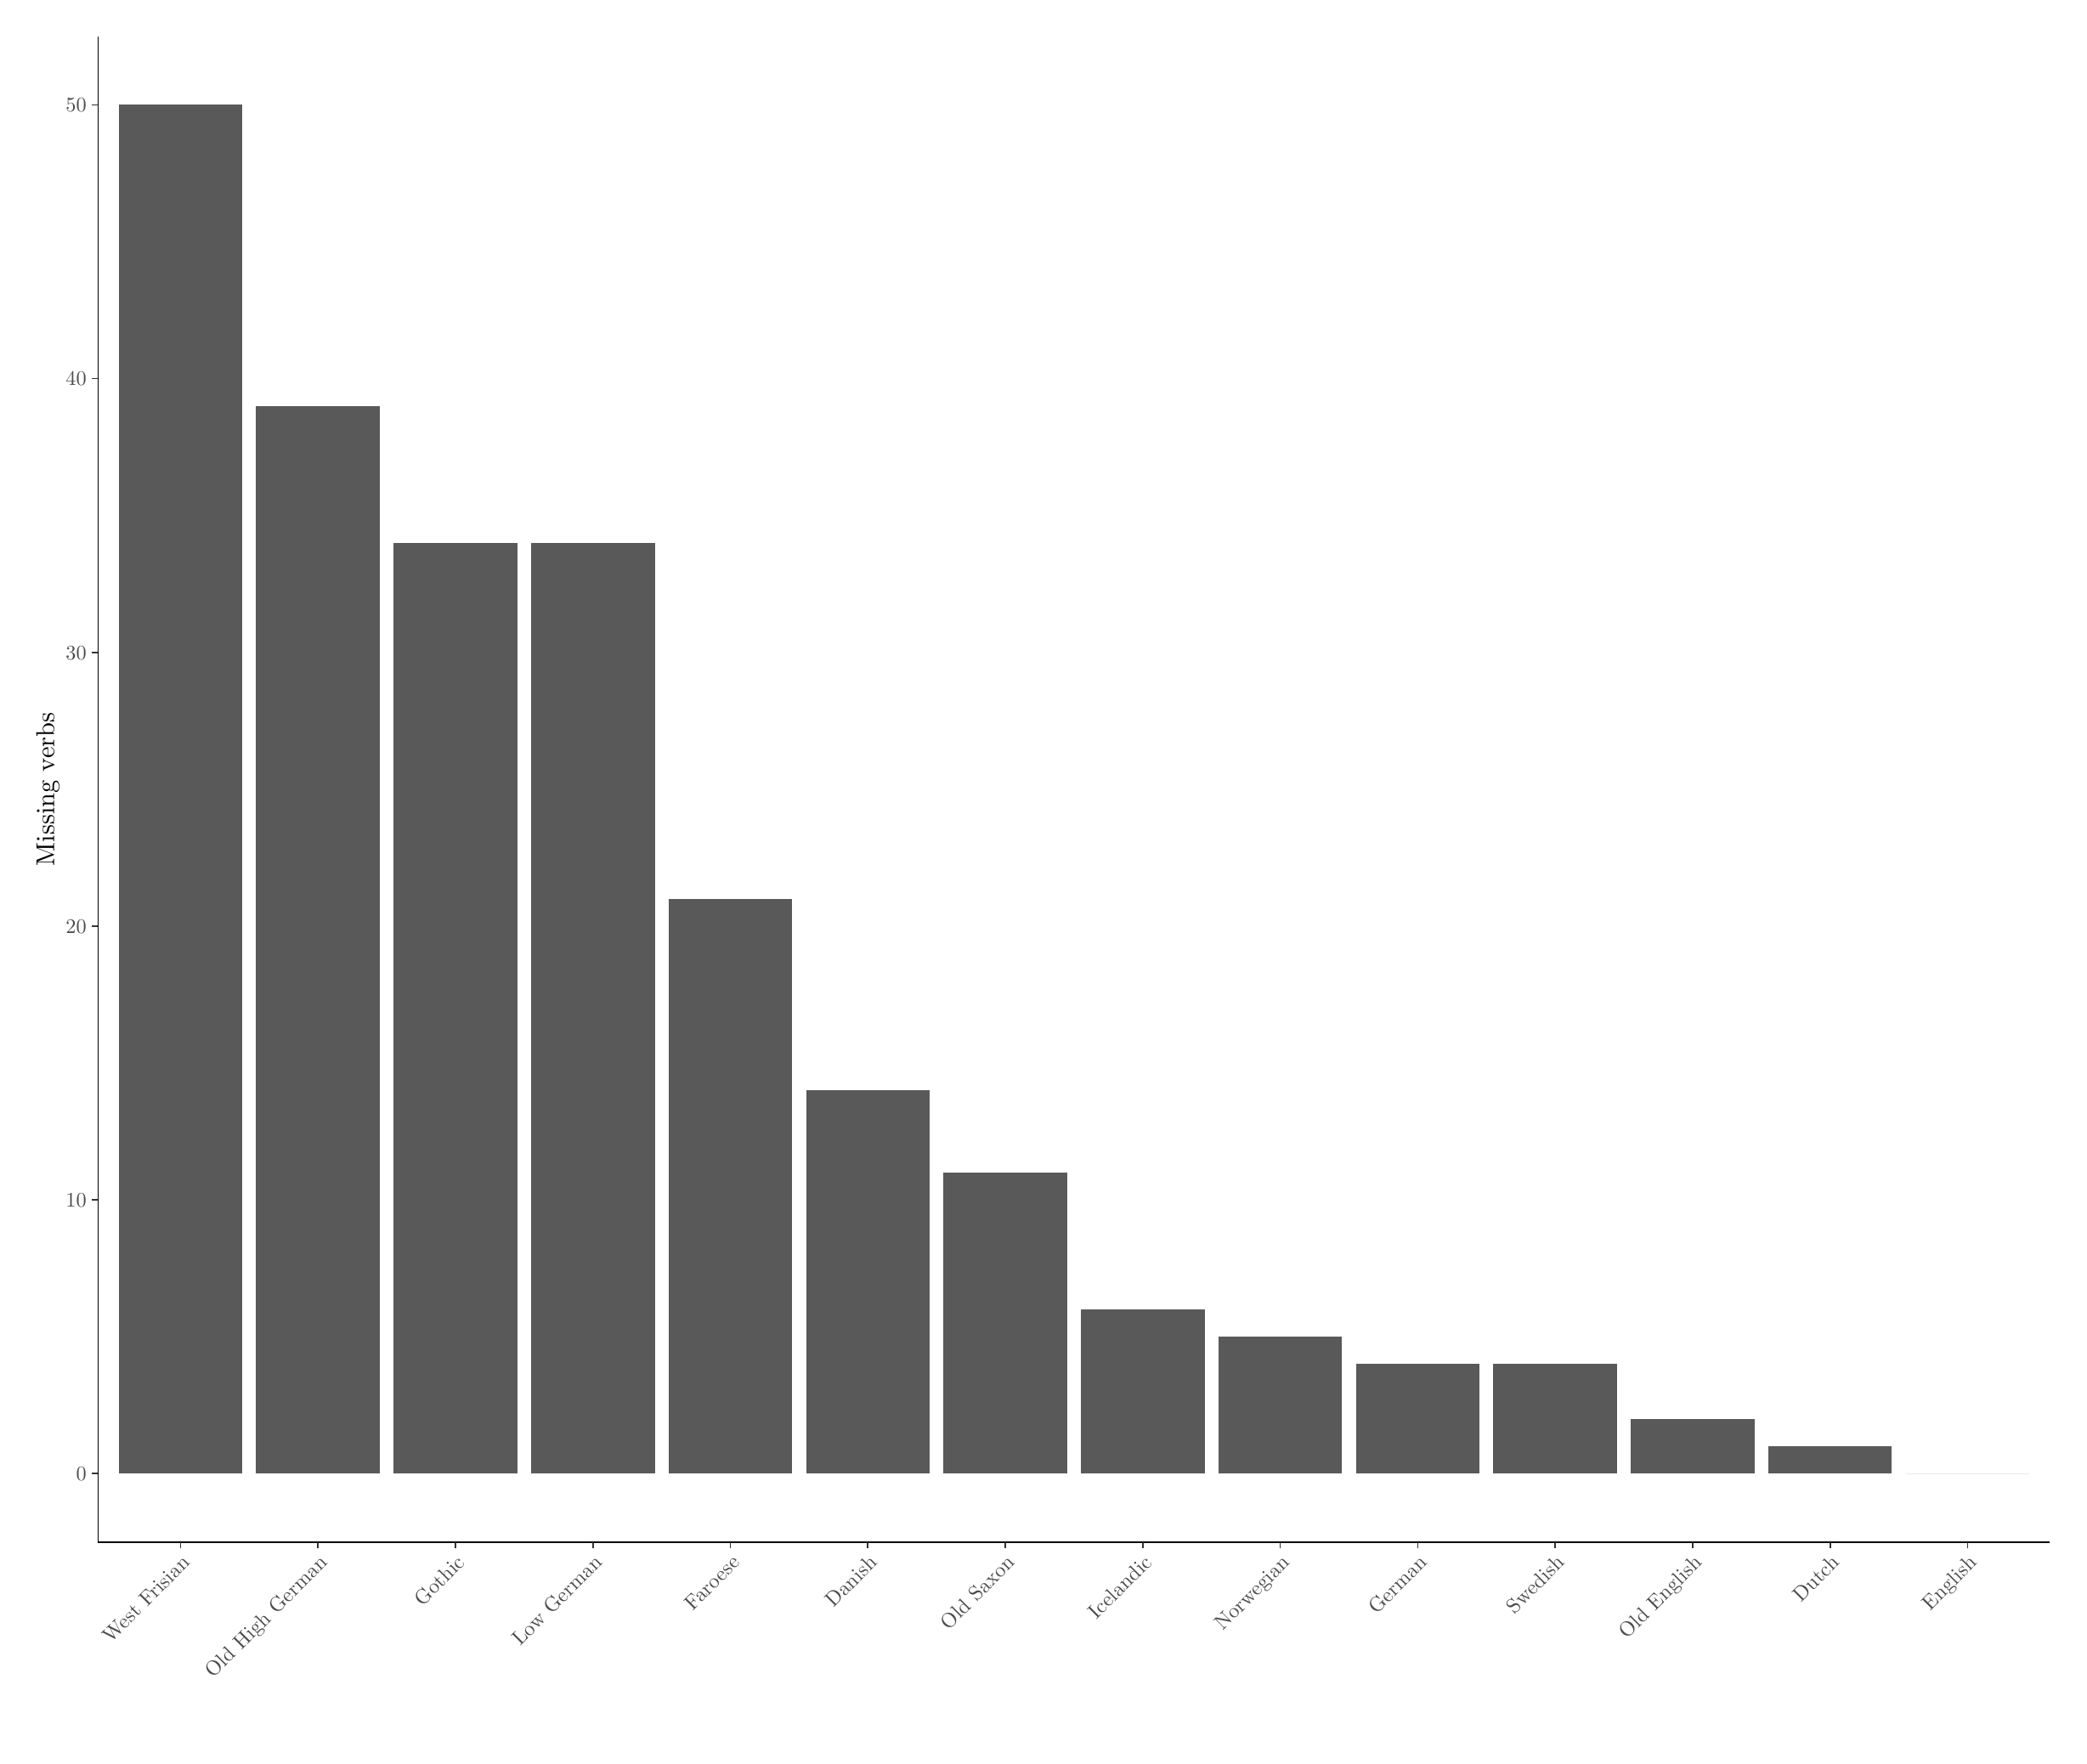
\begin{tikzpicture}[x=1pt,y=1pt]
\definecolor{fillColor}{RGB}{255,255,255}
\path[use as bounding box,fill=fillColor,fill opacity=0.00] (0,0) rectangle (867.24,729.93);
\begin{scope}
\path[clip] (  0.00,  0.00) rectangle (867.24,729.93);
\definecolor{drawColor}{RGB}{255,255,255}
\definecolor{fillColor}{RGB}{255,255,255}

\path[draw=drawColor,line width= 0.6pt,line join=round,line cap=round,fill=fillColor] (  0.00,  0.00) rectangle (867.24,729.93);
\end{scope}
\begin{scope}
\path[clip] ( 31.71, 84.16) rectangle (861.74,724.43);
\definecolor{fillColor}{RGB}{255,255,255}

\path[fill=fillColor] ( 31.71, 84.16) rectangle (861.74,724.43);
\definecolor{fillColor}{gray}{0.35}

\path[fill=fillColor] ( 40.48,113.26) rectangle ( 93.09,695.32);

\path[fill=fillColor] ( 98.93,113.26) rectangle (151.54,567.27);

\path[fill=fillColor] (157.39,113.26) rectangle (209.99,509.06);

\path[fill=fillColor] (215.84,113.26) rectangle (268.45,509.06);

\path[fill=fillColor] (274.29,113.26) rectangle (326.90,357.73);

\path[fill=fillColor] (332.74,113.26) rectangle (385.35,276.24);

\path[fill=fillColor] (391.20,113.26) rectangle (443.80,241.31);

\path[fill=fillColor] (449.65,113.26) rectangle (502.26,183.11);

\path[fill=fillColor] (508.10,113.26) rectangle (560.71,171.47);

\path[fill=fillColor] (566.55,113.26) rectangle (619.16,159.83);

\path[fill=fillColor] (625.01,113.26) rectangle (677.61,159.83);

\path[fill=fillColor] (683.46,113.26) rectangle (736.07,136.54);

\path[fill=fillColor] (741.91,113.26) rectangle (794.52,124.90);

\path[fill=fillColor] (800.36,113.26) rectangle (852.97,113.26);
\end{scope}
\begin{scope}
\path[clip] (  0.00,  0.00) rectangle (867.24,729.93);
\definecolor{drawColor}{RGB}{0,0,0}

\path[draw=drawColor,line width= 0.6pt,line join=round] ( 31.71, 84.16) --
	( 31.71,724.43);
\end{scope}
\begin{scope}
\path[clip] (  0.00,  0.00) rectangle (867.24,729.93);
\definecolor{drawColor}{gray}{0.30}

\node[text=drawColor,anchor=base east,inner sep=0pt, outer sep=0pt, scale=  0.88] at ( 26.76,110.23) {0};

\node[text=drawColor,anchor=base east,inner sep=0pt, outer sep=0pt, scale=  0.88] at ( 26.76,226.64) {10};

\node[text=drawColor,anchor=base east,inner sep=0pt, outer sep=0pt, scale=  0.88] at ( 26.76,343.06) {20};

\node[text=drawColor,anchor=base east,inner sep=0pt, outer sep=0pt, scale=  0.88] at ( 26.76,459.47) {30};

\node[text=drawColor,anchor=base east,inner sep=0pt, outer sep=0pt, scale=  0.88] at ( 26.76,575.88) {40};

\node[text=drawColor,anchor=base east,inner sep=0pt, outer sep=0pt, scale=  0.88] at ( 26.76,692.29) {50};
\end{scope}
\begin{scope}
\path[clip] (  0.00,  0.00) rectangle (867.24,729.93);
\definecolor{drawColor}{gray}{0.20}

\path[draw=drawColor,line width= 0.6pt,line join=round] ( 28.96,113.26) --
	( 31.71,113.26);

\path[draw=drawColor,line width= 0.6pt,line join=round] ( 28.96,229.67) --
	( 31.71,229.67);

\path[draw=drawColor,line width= 0.6pt,line join=round] ( 28.96,346.09) --
	( 31.71,346.09);

\path[draw=drawColor,line width= 0.6pt,line join=round] ( 28.96,462.50) --
	( 31.71,462.50);

\path[draw=drawColor,line width= 0.6pt,line join=round] ( 28.96,578.91) --
	( 31.71,578.91);

\path[draw=drawColor,line width= 0.6pt,line join=round] ( 28.96,695.32) --
	( 31.71,695.32);
\end{scope}
\begin{scope}
\path[clip] (  0.00,  0.00) rectangle (867.24,729.93);
\definecolor{drawColor}{RGB}{0,0,0}

\path[draw=drawColor,line width= 0.6pt,line join=round] ( 31.71, 84.16) --
	(861.74, 84.16);
\end{scope}
\begin{scope}
\path[clip] (  0.00,  0.00) rectangle (867.24,729.93);
\definecolor{drawColor}{gray}{0.20}

\path[draw=drawColor,line width= 0.6pt,line join=round] ( 66.78, 81.41) --
	( 66.78, 84.16);

\path[draw=drawColor,line width= 0.6pt,line join=round] (125.24, 81.41) --
	(125.24, 84.16);

\path[draw=drawColor,line width= 0.6pt,line join=round] (183.69, 81.41) --
	(183.69, 84.16);

\path[draw=drawColor,line width= 0.6pt,line join=round] (242.14, 81.41) --
	(242.14, 84.16);

\path[draw=drawColor,line width= 0.6pt,line join=round] (300.59, 81.41) --
	(300.59, 84.16);

\path[draw=drawColor,line width= 0.6pt,line join=round] (359.05, 81.41) --
	(359.05, 84.16);

\path[draw=drawColor,line width= 0.6pt,line join=round] (417.50, 81.41) --
	(417.50, 84.16);

\path[draw=drawColor,line width= 0.6pt,line join=round] (475.95, 81.41) --
	(475.95, 84.16);

\path[draw=drawColor,line width= 0.6pt,line join=round] (534.41, 81.41) --
	(534.41, 84.16);

\path[draw=drawColor,line width= 0.6pt,line join=round] (592.86, 81.41) --
	(592.86, 84.16);

\path[draw=drawColor,line width= 0.6pt,line join=round] (651.31, 81.41) --
	(651.31, 84.16);

\path[draw=drawColor,line width= 0.6pt,line join=round] (709.76, 81.41) --
	(709.76, 84.16);

\path[draw=drawColor,line width= 0.6pt,line join=round] (768.22, 81.41) --
	(768.22, 84.16);

\path[draw=drawColor,line width= 0.6pt,line join=round] (826.67, 81.41) --
	(826.67, 84.16);
\end{scope}
\begin{scope}
\path[clip] (  0.00,  0.00) rectangle (867.24,729.93);
\definecolor{drawColor}{gray}{0.30}

\node[text=drawColor,rotate= 45.00,anchor=base east,inner sep=0pt, outer sep=0pt, scale=  0.88] at ( 71.07, 74.92) {West Frisian};

\node[text=drawColor,rotate= 45.00,anchor=base east,inner sep=0pt, outer sep=0pt, scale=  0.88] at (129.52, 74.92) {Old High German};

\node[text=drawColor,rotate= 45.00,anchor=base east,inner sep=0pt, outer sep=0pt, scale=  0.88] at (187.97, 74.92) {Gothic};

\node[text=drawColor,rotate= 45.00,anchor=base east,inner sep=0pt, outer sep=0pt, scale=  0.88] at (246.43, 74.92) {Low German};

\node[text=drawColor,rotate= 45.00,anchor=base east,inner sep=0pt, outer sep=0pt, scale=  0.88] at (304.88, 74.92) {Faroese};

\node[text=drawColor,rotate= 45.00,anchor=base east,inner sep=0pt, outer sep=0pt, scale=  0.88] at (363.33, 74.92) {Danish};

\node[text=drawColor,rotate= 45.00,anchor=base east,inner sep=0pt, outer sep=0pt, scale=  0.88] at (421.79, 74.92) {Old Saxon};

\node[text=drawColor,rotate= 45.00,anchor=base east,inner sep=0pt, outer sep=0pt, scale=  0.88] at (480.24, 74.92) {Icelandic};

\node[text=drawColor,rotate= 45.00,anchor=base east,inner sep=0pt, outer sep=0pt, scale=  0.88] at (538.69, 74.92) {Norwegian};

\node[text=drawColor,rotate= 45.00,anchor=base east,inner sep=0pt, outer sep=0pt, scale=  0.88] at (597.14, 74.92) {German};

\node[text=drawColor,rotate= 45.00,anchor=base east,inner sep=0pt, outer sep=0pt, scale=  0.88] at (655.60, 74.92) {Swedish};

\node[text=drawColor,rotate= 45.00,anchor=base east,inner sep=0pt, outer sep=0pt, scale=  0.88] at (714.05, 74.92) {Old English};

\node[text=drawColor,rotate= 45.00,anchor=base east,inner sep=0pt, outer sep=0pt, scale=  0.88] at (772.50, 74.92) {Dutch};

\node[text=drawColor,rotate= 45.00,anchor=base east,inner sep=0pt, outer sep=0pt, scale=  0.88] at (830.95, 74.92) {English};
\end{scope}
\begin{scope}
\path[clip] (  0.00,  0.00) rectangle (867.24,729.93);
\definecolor{drawColor}{RGB}{0,0,0}

\node[text=drawColor,rotate= 90.00,anchor=base,inner sep=0pt, outer sep=0pt, scale=  1.10] at ( 13.08,404.29) {Missing verbs};
\end{scope}
\end{tikzpicture}
